\documentclass{beamer}

\usepackage{graphicx}
\usepackage{amsmath}

\title{Week 3 CUSF Controls Introductory Project - Linearisation and PID}
\author{Yoonjae Hwang}
\date{26 October 2025}

\begin{document}
\frame{\titlepage}

\title{Part 1: Linearisation methods}
\begin{frame}
\maketitle
\end{frame}

\begin{frame}
\frametitle{Motivating Example - Inverted Pendulum on a Cart}

\begin{columns}
    \begin{column}{0.7\textwidth}
        Horizontally (cart):
        \begin{equation}
            M \ddot{x} + N = F
        \end{equation}
        Horizontally (rod):
        \begin{equation}
            N = m \ddot{x} + ml \ddot{\theta} \sin{\theta}- m l \dot{\theta}^2 \sin(\theta)
        \end{equation}
        $(2) \to (1)$:
        \begin{equation}
            (M+m)\ddot{x} + ml \ddot{\theta} \cos(\theta) - ml \dot{\theta}^2 \sin(\theta) = F(t)
        \end{equation}
    \end{column}
    \begin{column}{0.3\textwidth}
        \centering
        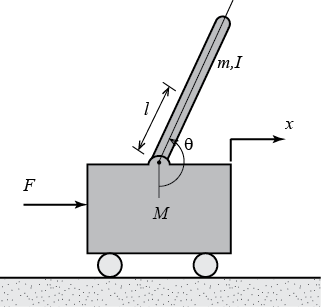
\includegraphics[width=\textwidth]{invpend.png}
    \end{column}
\end{columns}

\end{frame}

\begin{frame}
\frametitle{Continued}
Considering the torque on the rod: 
\begin{equation}
    Pl \sin(\theta) - Nl\cos(theta) - I \ddot{\theta} = 0
\end{equation}
Forces perpendicular to rod: 
\begin{equation}
    N \cos(\theta) - P \sin(\theta) - m l \ddot{\theta} - m \ddot{x} \cos(\theta) + mg \sin(\theta) = 0
\end{equation}
$(4) \to (5)$ and simplifying: 
\begin{equation}
    (I + ml^2) \ddot{\theta} + ml \ddot{x} \cos{\theta} - mgl sin{\theta} = 0  
\end{equation}

\end{frame}

\begin{frame}
\frametitle{Resulting Equations of Motion}
So overall, our system of nonlinear equations of motion is: 
\begin{equation}
    (M+m)\ddot{x} + ml \ddot{\theta} \cos(\theta) - ml \dot{\theta}^2 \sin(\theta) = F(t)
\end{equation}

\begin{equation}
    (I + ml^2) \ddot{\theta} + ml \ddot{x} \cos{\theta} - mgl sin{\theta} = 0  
\end{equation}
One may now rearrange this into a first order differential equation in state space form. 
It may be of interest to explore what the behaviour is around the equilibrium point ($\theta = 0$).
To do this we may linearise the equations by using small angle approximations.
\end{frame}

\begin{frame}
\frametitle{MATLAB Implementation of the system}
\begin{center}
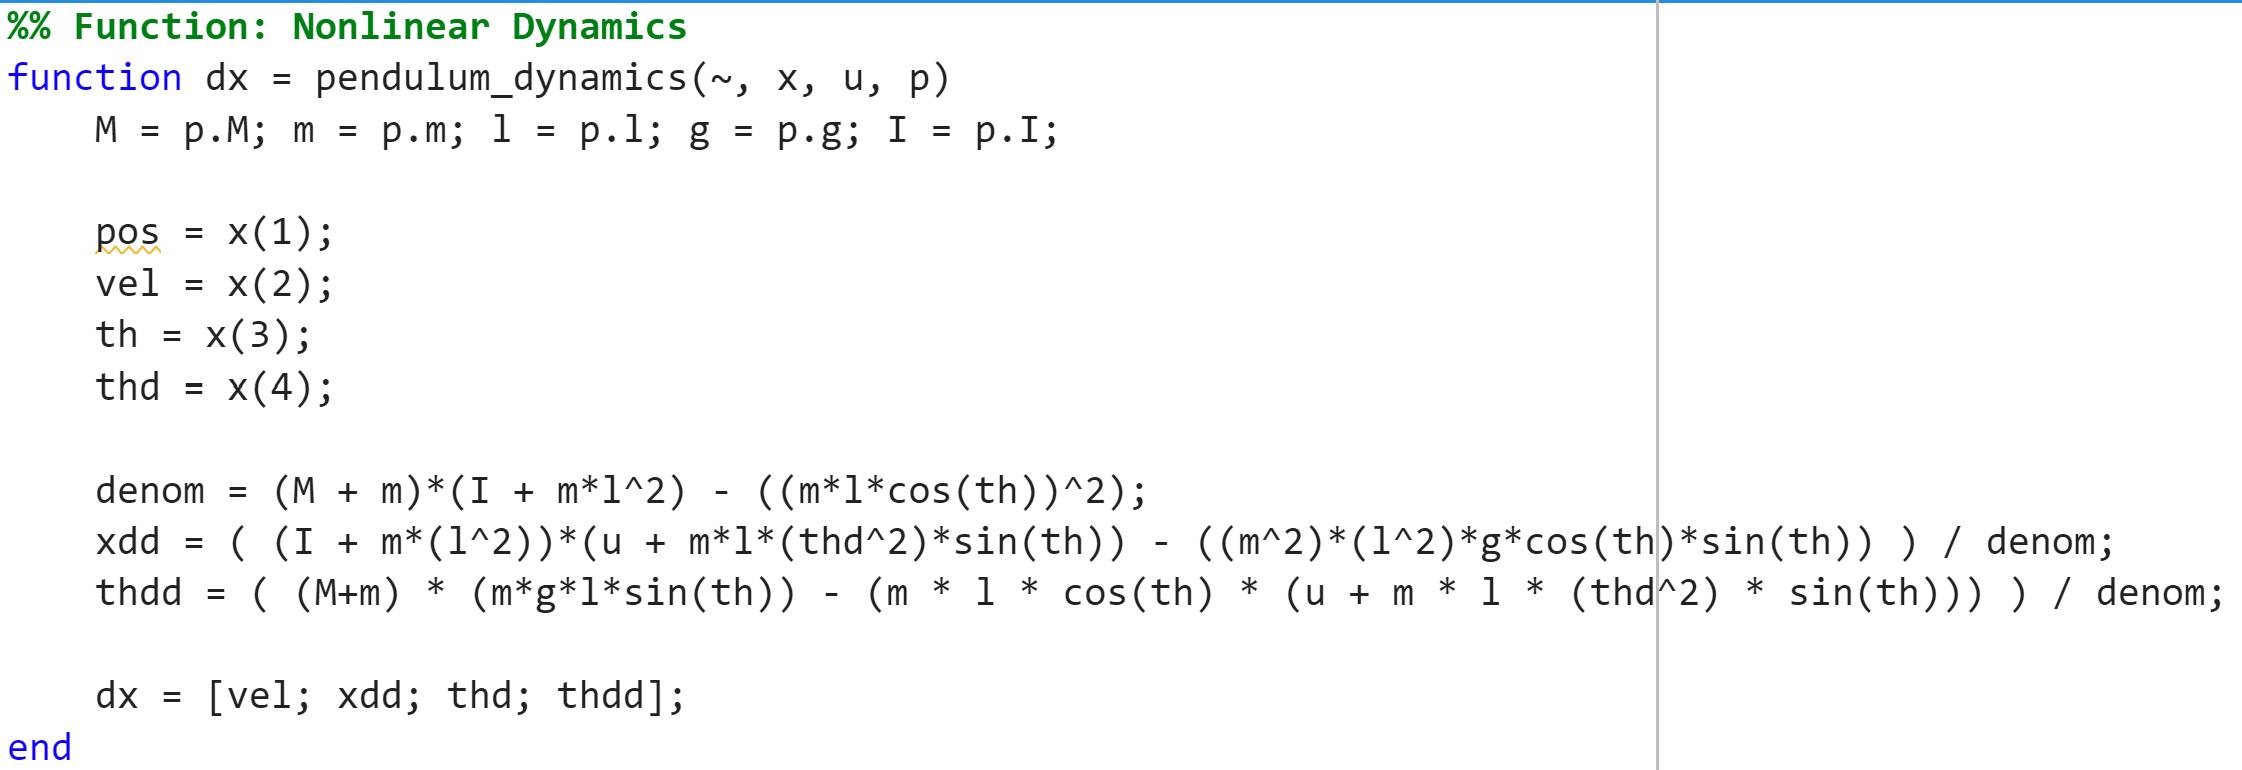
\includegraphics[width = 0.9\textwidth]{matlab_sim.png}
\end{center}
\end{frame}

\begin{frame}
\frametitle{Linearising with Small Angle Approximation}
For small $\theta$:
\begin{equation}
    \cos(\theta) \approx 1, \space \sin(\theta) \approx \theta
\end{equation}

So the resulting equations of motion become: 
\begin{equation}
    (M+m)\ddot{x} + ml \ddot{\theta} = F(t)
\end{equation}

\begin{equation}
    (I + ml^2) \ddot{\theta} + ml \ddot{x} - mgl \theta = 0  
\end{equation}

\end{frame}

\begin{frame}
\frametitle{General Systems}
For a general nonlinear system:
\begin{equation}
    \dot{x} = f(x, u)
\end{equation}
And the equilibrium points being $(x_e, u_e)$.
We consider the Taylor expansion of $f(x, u)$ up to the first order derivative:
\begin{equation}
    f(x, u) = f(x_e, u_e) 
    + \left.\frac{\partial f}{\partial x}\right|_{x = x_e} (x - x_e) 
    + \left.\frac{\partial f}{\partial u}\right|_{u = u_e} (u - u_e)
\end{equation}
The partial derivatives $\left.\frac{\partial f}{\partial x}\right|_{x = x_e}$, and $\left.\frac{\partial f}{\partial u}\right|_{u = u_e}$
are matrices of partial derivatives of every component of f with every component of x, u respectively.
The matrix is called the Jacobian. 
\end{frame}

\begin{frame}
\frametitle{Continued}
We then define new variables of state, $\tilde{x} = x - x_e$ and $\tilde{u} = u - u_e$.
Then we can write the equations of motion: 
\begin{equation}
    \dot{\tilde{x}} = A \tilde{x} + B \tilde{u} 
\end{equation}
where $A = \left.\frac{\partial f}{\partial x}\right|_{x = x_e}$, and $B = \left.\frac{\partial f}{\partial u}\right|_{u = u_e}$. 
Now with a linear approximation of the system, the tools developed for linear controller/observer design can be used 
(LQR, Pole placement, Linear MPC, etc).

\end{frame}

\begin{frame}
    \begin{center}
        \includegraphics[width = 0.8\textwidth]{linearisation2.png}
    \end{center}
\end{frame}


%% PID %%
\title{Part 2: Introduction to PID Control}
\begin{frame}
\maketitle
\end{frame}

\begin{frame}
\frametitle{On-Off Control}
\begin{equation}
u = 
\begin{cases}
    u_{max} & \text{if } e > 0\\
    u_{min} & \text{if } e < 0
\end{cases}
\end{equation}
\begin{itemize}
    \item $e = r - y$
    \item Simplest control system
    \item Control variable oscillates - might be acceptable if small enough
    \item Control not defined when error is 0
    \item System overreacts to a small change in error
\end{itemize}
\end{frame}

\begin{frame}
\frametitle{Proportional (P) Control}
\begin{equation}
u = 
\begin{cases}
    u_{max} & \text{if } e \geq e_{max}\\
    k_p e & \text{if } e_{min} < e < e_{max} \\
    u_{min} & \text{if } e \leq e_{min} 
\end{cases}
\end{equation}
\begin{itemize}
    \item Controller input is proportional to the control error for small errors
    \item Might be enough
    \item Drawbacks: deviates from its reference value - prone to steady state error when there is a steady disturbance
    \item We want the error to go to 0 over time
\end{itemize}
\end{frame}

\begin{frame}
\frametitle{Proportional-Integral Control (PI)}
\begin{equation}
u = k_p e + k_I \int_{0}^{t} e(\tau) d\tau
\end{equation}
\begin{itemize}
    \item We want to track the error during the course of the system's motion
    \item Sum the error at each step - ie integration
    \item Drawbacks: steady-state may not be always present
    \item If we have magnitude limits - integrator windup can occur
    \item Careful design and analysis needed
\end{itemize}
\end{frame}

\begin{frame}
\frametitle{Proportional-Integral-Derivative Control (PID)}
\begin{equation}
u = k_p e + k_I \int_{0}^{t} e(\tau) d\tau + k_D \dot{e}(t)
\end{equation}
\begin{itemize}
    \item Derivative term increases the damping
    \item Provides information where the error is heading - linear extrapolation of the error
    \item Helps correct overshoot
    \item Prone to noise - which can result in controller being unstable, reducing robustness
\end{itemize}
\end{frame}

\begin{frame}
\begin{center}
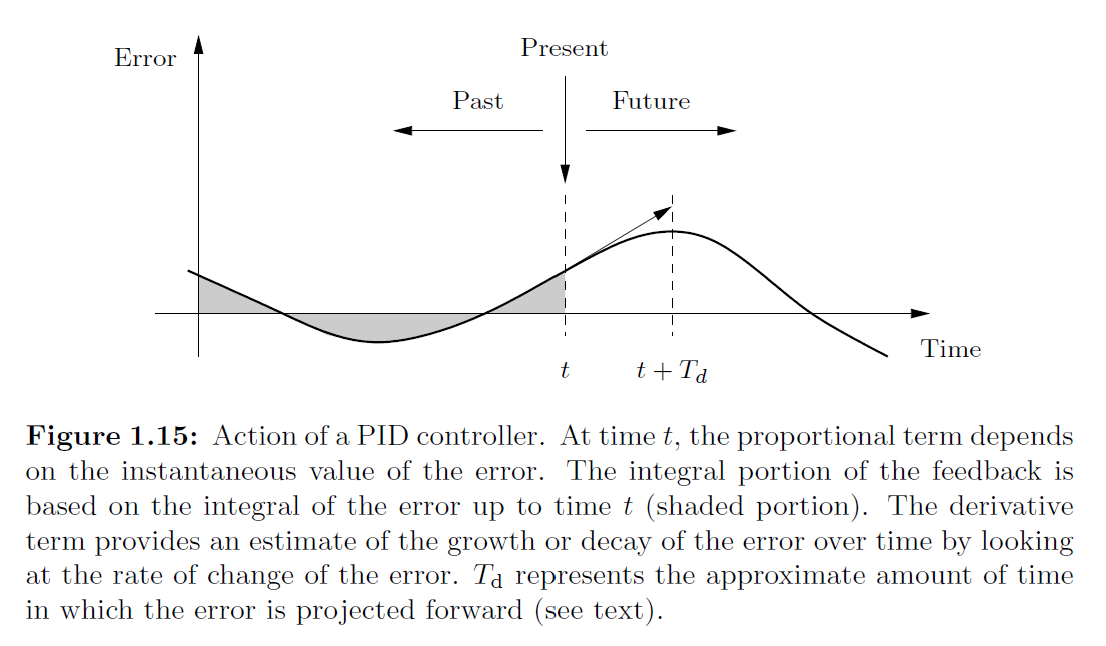
\includegraphics[width = 1.0\textwidth]{PIDdiagram.png}
\end{center}
\end{frame}

\begin{frame}
\frametitle{TASK}
\begin{itemize}
    \item Modelling a 3DOF Thrust vectored rocket
    \item Obtain nonlinear equations of motion
    \item Linearise and obtain linear state space equation of motion
    \item Produce a Simulink diagram for it
\end{itemize}
\end{frame}

\begin{frame}
\frametitle{Next 2 Weeks}
\begin{itemize}
    \item State Feedback
    \item Linear Quadratic Regulators
    \item Pole placement
    \item Controllability
\end{itemize}
\end{frame}


\end{document}